% Chapter Template

\chapter{Background Theory} % Main chapter title

\label{Chapter3} % Change X to a consecutive number; for referencing this chapter elsewhere, use \ref{ChapterX}
Localization systems come with various architectures and system designs. Several different methodologies can be applied to estimate the targets current position. In this chapter we distinguish between client and server-based system architectures. We introduce fingerprinting-based and range-based localization techniques, as well as the principles of movement detection. The process of information fusion from different data sources and the radio technology of ultra wideband is explained in the last two sections.

%----------------------------------------------------------------------------------------
%	SECTION 1
%----------------------------------------------------------------------------------------
\section{Client and Server-based Localization}
For many applications the system architecture is very important. The environmental conditions, the underlying hardware and also dogmatic thoughts are taken into account for real applications to determine the system architecture. There are two main types of system architectures - client-based or server-based - that can be distinguished. However, systems using computational resources of client and servers are possible, where a clear distinction is no longer possible.\\
\noindent\hspace*{5mm}%
Client-based architectures have the huge advantage, that no additional server hardware is needed. The client device collects data used for the localization and processes it, to estimate its own position. A client-based localization should be used when standardized target devices with enough computational power and enough energy supply are localized. As all computations are done on the device itself, no further communication to a seperated server is needed. This ensures that no other application can access the position estimation and reduces the communication overhead.\\
\noindent\hspace*{5mm}%
A server-based system however, can be more powerful and computationally complex than client-based systems, as there are no big hardware restrictions. The application itself runs on a seperate server, whereas the client-device is only involved in the data collection process. The requirements of the client-hardware shrink to a minimum, which allows also to use different, non-standardized, devices as target. Especially when position estimations are not used in applications running on the target device, a server-based architecture is beneficial because data of several target devices is available and can be further used on the server or in cloud applications. 


%----------------------------------------------------------------------------------------
%	SECTION 2
%----------------------------------------------------------------------------------------
\section{Fingerprinting Localization Technique}
Fingerprinting Localization, also known as radio map based technique, use a dense positioning of anchor nodes in the indoor area. A set of measurements, often received signal strength measurements, serve as a fingerprint at each location. Measurments are not limited to radio signals, other sources such as magnetic field data can also be used. The more unique these measurements are, the better is the localization accuracy. Fingerprinting often consists of an offline phase to generate the radio map and an online phase to retrieve the position with a given fingerprint.\\
\noindent\hspace*{5mm}%
In the offline phase, a radio map is generated with several fingerprints. The radio map can either consist of different fingerprint measurements at given reference points (landmarks) that are interpolated to the whole area, or of fingerprints measured in predefined zones in the area of interest. After this phase, for every location in the grid, a tupel (location, fingerprint) with a unique fingerprint should be available.\\
\noindent\hspace*{5mm}%
The online phase consists of an observed fingerprint at the targets location, on which the localization algorithm can be applied to associate the fingerprint to simliar radio map entries. This association is then used to estimate the targets location. The result can either be a concrete position estimation built on the presence of reference points or it can be a probability of the target being in a recognized zone. 

%----------------------------------------------------------------------------------------
%	SECTION 1
%----------------------------------------------------------------------------------------

\section{Range Based Localization}

Range based localization systems are depending on an infrastructure in the area of the localization:
\begin{itemize} 
\item \textbf{Target Node (TAG)} which is the device that is localized. 
\item \textbf{Anchor Nodes (AN)} that are placed on carefully chosen points in the building, to encounter the best coverage of the whole area.
\end{itemize}

The key idea of range based positioning is to measure the distance between TAG and ANs. With the use of these distances, the exact position of the TAG can be evaluated using multilateration or similar mathematical models. Several different approaches are possible to determine the distance to an anchor node, they can be classified into the two groups. In the one hand there are algorithms using propagation models, which rely on the reduction in power density of electromagnetic waves propagating through space. In the other hand, algorithms make use of known propagation velocities for radio signals  by measuring the time of flight of transmitted waves. 

%-----------------------------------
%	SUBSECTION 1
%-----------------------------------
\subsection{Propagation Models}
An electromagnetic wave loses power density when travelling through space. In free space, the following formula explains the relationship between distance and signal strength \cite{VorlesungCN}.

\begin{equation}
P_{r} = P_{t} (\lambda/4\pi r)^2
\label{eqn:freePathLoss}
\end{equation}

where $P_{r}$ is the received signal strength and $P_{t}$ the transmitted signal strength. $\lambda$ is the wavelength and $r$ the radius, or in other words the distance from transmitter to receiver. As this formula is restricted to free-space and often in real indoor environments various kind of obstacles are present, several other approximations for the relationship between distance and signal power exist. Many indoor positioning algorithms use received signal strength indication (RSSI) to calculate distances to the anchor nodes. Mainly because RSSI can be applied to almost every type of transmitted signal, thus RSSI uses universal applicable theory. Two approximations are widely used to take care of the non-free-space environments indoors.\\
\noindent\hspace*{5mm}%
A commonly used model for the relationship of distance and RSS is known as Log-normal Distance Path Loss (LDPL), where the path loss in Decibel (dB) is defined as \cite{Sarkar}:
\begin{equation}
PL = PL_{0} +10 \gamma log_{10} (\frac{d}{d_{0}}) + X_{g}
\label{eqn:LDPL}
\end{equation}

with $\gamma$ as the path loss exponent, $PL_{0}$ a path loss measurement at reference distance $d_0$ and $X_{g}$ a zero-mean Gaussian noise. This generic model can be applied to many different enviroments. It can even be simplified by defining useful reference distances, like done in \cite{Kurt}.\\
\noindent\hspace*{5mm}%
LDPL has shown to be rather inaccurate for indoor environments, which led to a path loss model based on Non-Linear Regression (NLR) as used in \cite{ZanLi}. In this approach, the distance to RSS relationship is modelled with the equation:
\begin{equation}
d_{i} = \alpha_{i} e^{\beta_{i}RSS_{i}}.
\label{eqn:NLR}
\end{equation}
$d_{i}$ is the distance between the $i$-th AN and the TAG, $RSS_{i}$ the measured signal strength at the $i$-th AN and $\alpha_{i}$, $\beta_{i}$ specific coefficients obtained in the area of interest. These two coefficients are rather important for the performance of this approach. They are defined due to extensive calculations based on preliminary measuements as described in \cite{Kurt}.


%-----------------------------------
%	SUBSECTION 2
%-----------------------------------
\subsection{Time of Flight Based Models}
Gathering round trip times (RTT) is a second method to get distance estimations. For accurate RTT results the hardware of transmitter and receiver, as well as the operating firmware are very important. For the presented two RTT-measuring communication techniques, the key characteristics are either a quick responding time or extremely well synchronized TAG and AN.

\begin{figure}[th]
\centering
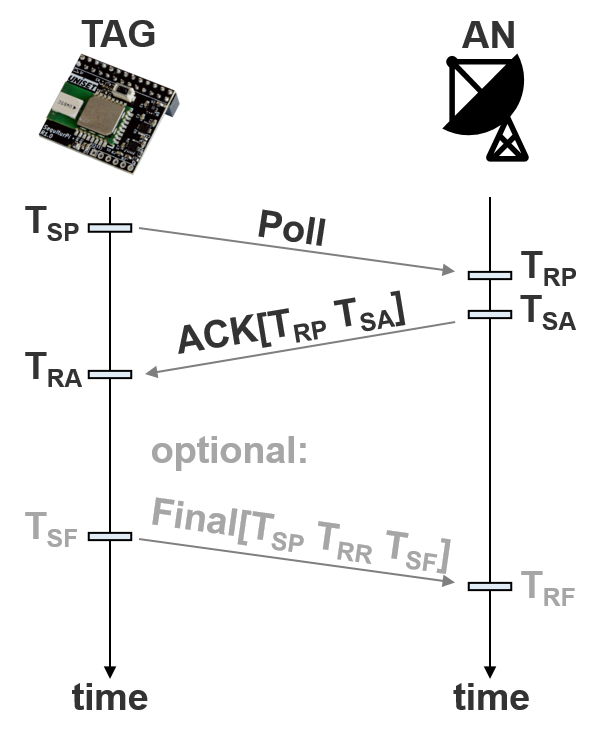
\includegraphics[width=0.5\textwidth]{Figures/two_way_ranging}
\decoRule
\caption[Two way ranging]{Illustration of TWR and SDS-TWR communication}
\label{fig:two_way_ranging}
\end{figure}

Operating in two way ranging (TWR) mode, the TAG sends a message to the ANs and registers the exact time of sending. As soon as the message arrives at its destination, the firmware of the AN instantly captures another timestamp. In an acknowledgement (ACK) message, the timestamp of reception and a timestamp of sending the response is transmitted. When this message arrives at the TAG, again a timestamp is registered. With the equation below, the time of flight can now be evaluated \cite{SewioTWR}.
To achieve higher accuracy, the communication can be extended with a final message containing the timestamps of the requester. This is called symmetrical double-sided two-way ranging (SDS-TWR) \cite{Wikipedia} and is indicated as optional in Figure \ref{fig:two_way_ranging}.\\
\\
Time of flight for TWR:\\
$$ ToF = [(T_{RA}-T_{SP})-(T_{SA}-T_{RP})] / 2$$\\
Time of flight for SDS-TWR:\\
$$ ToF = [(T_{RA}-T_{SP})-(T_{SA}-T_{RP}) + (T_{RF}-T_{SA})-(T_{SF}-T_{RA}) ]/ 4$$\\
$ToF$ - Time of flight\\
$T_{SP}$ - sending of poll timestamp \\
$T_{RP}$ - reception of poll timestamp\\
$T_{SA}$ - sending of ACK timestamp \\
$T_{RA}$ - reception of ACK timestamp\\
$T_{SF}$ - sending of final timestamp \\
$T_{RF}$ - reception of final timestamp\\

For simplicity reasons, normally ranging systems are designed such that the TAG gets the final message of the TWR communication, as the TWR is done with several ANs. In this case the requested information - the distances to every AN - is already on one device and can be further processed. However, the TWR has not necessarily to be inizialized by the TAG - the receiver and the sender can easily be exchanged. When for example the computational power of the TAG is limited or the application runs on a separate server, we can imagine some benefits to trigger the TWR in the ANs and forward the collected data directly to the server.

While TWR does not need further synchronization between the devices, time difference of arrival (TDOA) requires a very precise synchronization of the anchor nodes. This is normally done by specifying a master node per three to five anchors. For bigger scenarios often multiple dedicated masters will send clock synchronizations every once in a while, such that every AN gets at least one sync package. It occurs as well that an anchor holds two differently synchronized times.
To evaluate the time of flight, a TAG in range will broadcast a blink message. Every AN that receives this blink, will capture a timestamp of the time of arrival (or when holding more than one synctime, capture multiple timestamps). These timestamps are forwarded to the server together with a synch ID and a blink transmitter identity. When a server received at least three timestamps with the same synch ID for a tagret device, it can perform the position and therefore the distance estimation.
A huge benefit of TDOA is the fact, that the tag only needs to send one blink message per timeinterval and will not have to communicate with every AN separately, as in TWR. This can be seen in figure \ref{fig:time_difference_of_arrival}. For TWR the overhead grows enourmous with every anchor and every tag that is added. For TDOA hundrets of TAGs can be tracked, whith only proportional overhead growth and much lower energy consumption for the TAG.\\
Number of messages sent in one iteration:\\
TWR:  $3 * n_{t} * n_{an}$\\
TDOA:  $n_{t}$\\
Where $n_{t}$ is the number of TAGs and $n_{an}$ is the number of anchor nodes \cite{SewioTDOA}.

\begin{figure}[th]
\centering
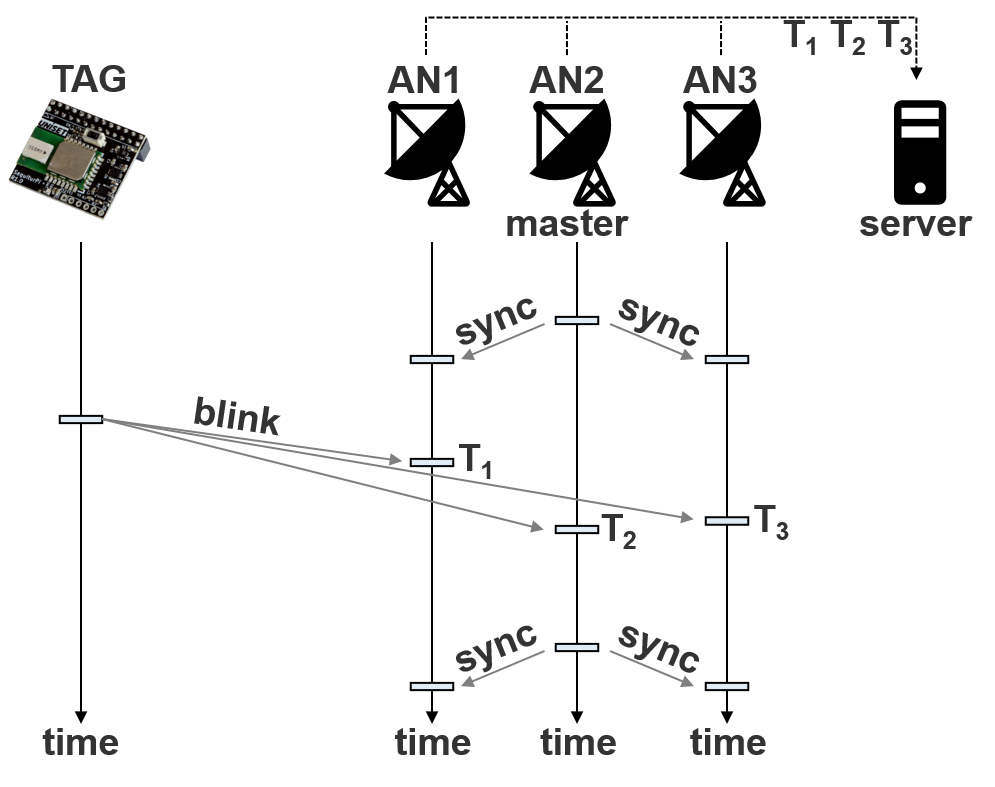
\includegraphics[width=0.7\textwidth]{Figures/time_difference_of_arrival}
\decoRule
\caption[Time difference of arrival]{Typical Setup for Time Difference of Arrival communication}
\label{fig:time_difference_of_arrival}
\end{figure}


For both methods the same calculations to convert the ToF to the related distance can be applied. We assume that radio signals travel almost with speed of light, so we just multiply the ToF with speed of light ($c_{0}$).
$$ distance = ToF * c_{0} $$\\
$ToF$ - Time of flight\\
$c_{0}$ - Speed of Light = \SI{2.99792458e8}{\meter\per\second} (exact) \\

%-----------------------------------
%	SUBSECTION 3
%-----------------------------------
\subsection{Triangulation and trilateration}
Triagulation and trilateration use the mathematical concepts of triangles to find unknown lengths. Triangulation was already mentioned by the greek mathematician Thales, who used this concept for finding out the height of ancient egypt pyramids \cite{thales}. It was also used for cartography purposes, where angles between fixed points were measured and heights and distances could be calculated. 
Although trilateration and triangulation use the same mathematical triangle concept, they have one defined difference: We call it triangulation, when angles to anchor positions are measured, otherwise - when distances to anchors are measured - it's called trilateration.
As it was easier to measure angles than distances in the past, triangulation was more often used. With modern electronic devices, it is more common to determine distances, rather than angles. 

Figure \ref{fig:trilateration} shows how trilateration is used for positioning. With the known distance to every AN, a circle with radius of this distance can be drawn around every AN. These circles do only have one common intersection point, that is where the TAG lies. However, this is a theoretical and idealized scenario, where every range can be determined accurately. In real applications, the ranges are not exactly calculated, what leads to the fact that we will not only get a single point for the calculated position, but several points, especially when we use more than three ANs.

\begin{figure}[th]
\centering
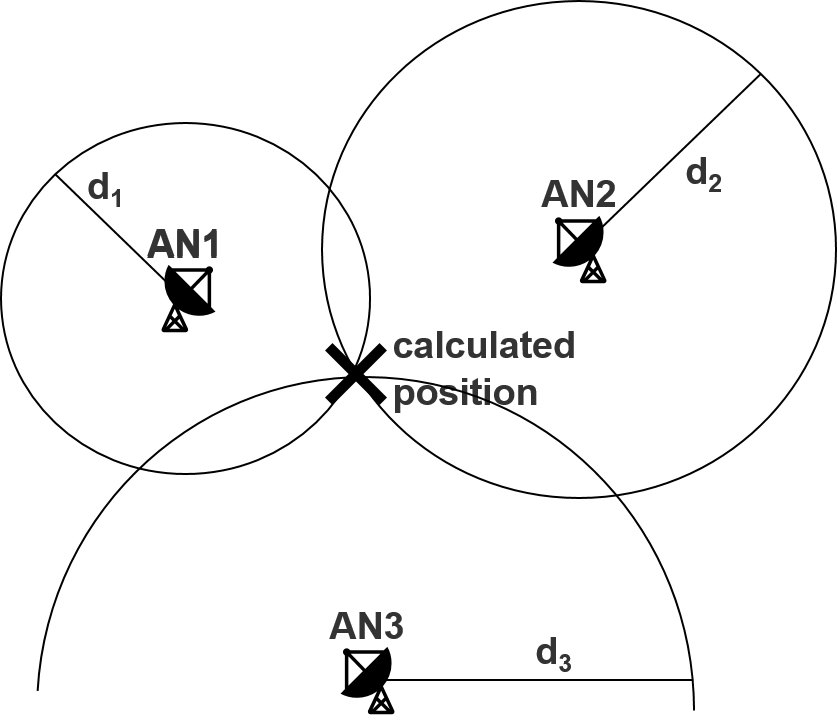
\includegraphics[width=0.6\textwidth]{Figures/trilateration}
\decoRule
\caption[Trilateration]{Graphical illustration of the trilateration concept.}
\label{fig:trilateration}
\end{figure}

%----------------------------------------------------------------------------------------
%	SECTION 2
%----------------------------------------------------------------------------------------

\section{UWB theory}
Ultra wide-band (UWB) is a radio technology in use for military communication, positioning and collecting sensor data. Unlike other communication technologies, UWB occupies a wide area of frequencies instead of just covering a small frequency spectrum. As showed in figure \ref{fig:frequency_spectrum}, UWB spans over a spectrum of more than 500 megahertz (MHz) that lies within the range of 3.1 gigahertz (GHz) and 13.6 GHz.
\begin{figure}[th]
\centering
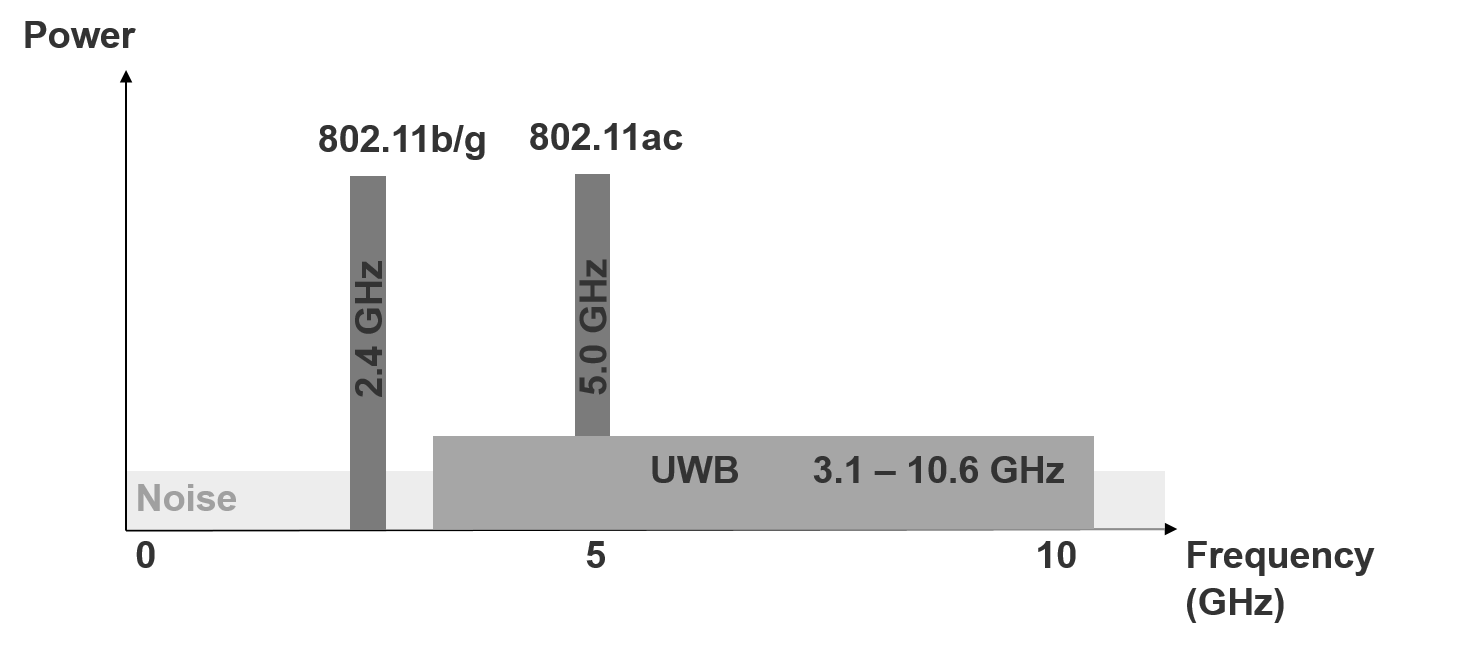
\includegraphics[width=1.0\textwidth]{Figures/frequency_spectrum}
\decoRule
\caption[UWB frequency spectrum]{Comparison of Wi-Fi (802.11) and UWB frequencies.}
\label{fig:frequency_spectrum}
\end{figure}
UWB opperates with less energy compared to other communication like Wi-Fi. However, the main difference between UWB and conventional radio transmissions is the underlying modulation technique. UWB transmits data by generating short radio energy at specific times instead of varying frequency and phase of sinus waves. In addition to the pulse position, the pulses can carry information either by their polarity, their amplitude or by using orthogonal pulses.
A single pulse is kept as short as possible, such that more than 100 Million, sometimes even continuous streams with more than 1 Billion pulses per second are generated. As single pulses can be registered and identified by the receiver, UWB devices are able to determine very exact ToFs such that distance estimations can be done to high resolution.


%----------------------------------------------------------------------------------------
%	SECTION 3
%----------------------------------------------------------------------------------------

\section{Particle filter and room recognition}

In the last years the CDS of UniBe has made big effort in developing an indoor positioning system. In various works, many variants of particle filter based localization have been presented and tested. In one of the latest works, the authors proposed a robust real-time indoor tracking system based on smartphones \cite{Carrera}, which extended some previous works \cite{Carrera3}. These works were mainly based on Wi-Fi RSSI measurements fusing with IMU data. Since there are no documentations about the particle filter approach based on UWB ranging, we will address this gap.\\
In addition, the CDS also presented enhanced machine learning techniques for room recognition based on Wi-Fi and magnetic field energy fingerprints \cite{Carrera2}.

As our work is an extension of the particle filter in combination with a simplified version of the room recognition algorithm, the principles of these works are explained in detail in chapter \ref{Chapter4}.